\section{Introduzione}
La presente tesi mira a studiare come cambia la vegetazione nel fiume Tagliamento in risposta al regime idrologico (successione di magre, piene bankfull, flood pulses). 
L'obiettivo principale è quello di ricercare una relazione tra i livelli del pelo libero registrati da un idrometro e la quantità di vegetazione presente in alveo, tra i livelli e la quantità di legname che si ritrova in alveo dopo eventi di piena.

Si analizzano immagini satellitari e ortofoto al fine di distinguere la parte dell'alveo ricoperta da vegetazione (\vref{fig:esempio-isola-1}) e gli elementi legnosi (tronchi e accumuli di legno, \vref{fig:esempio-accumulo-1}).

\begin{figure}
	\centering
	\begin{subfigure}[b]{0.37\textwidth}
		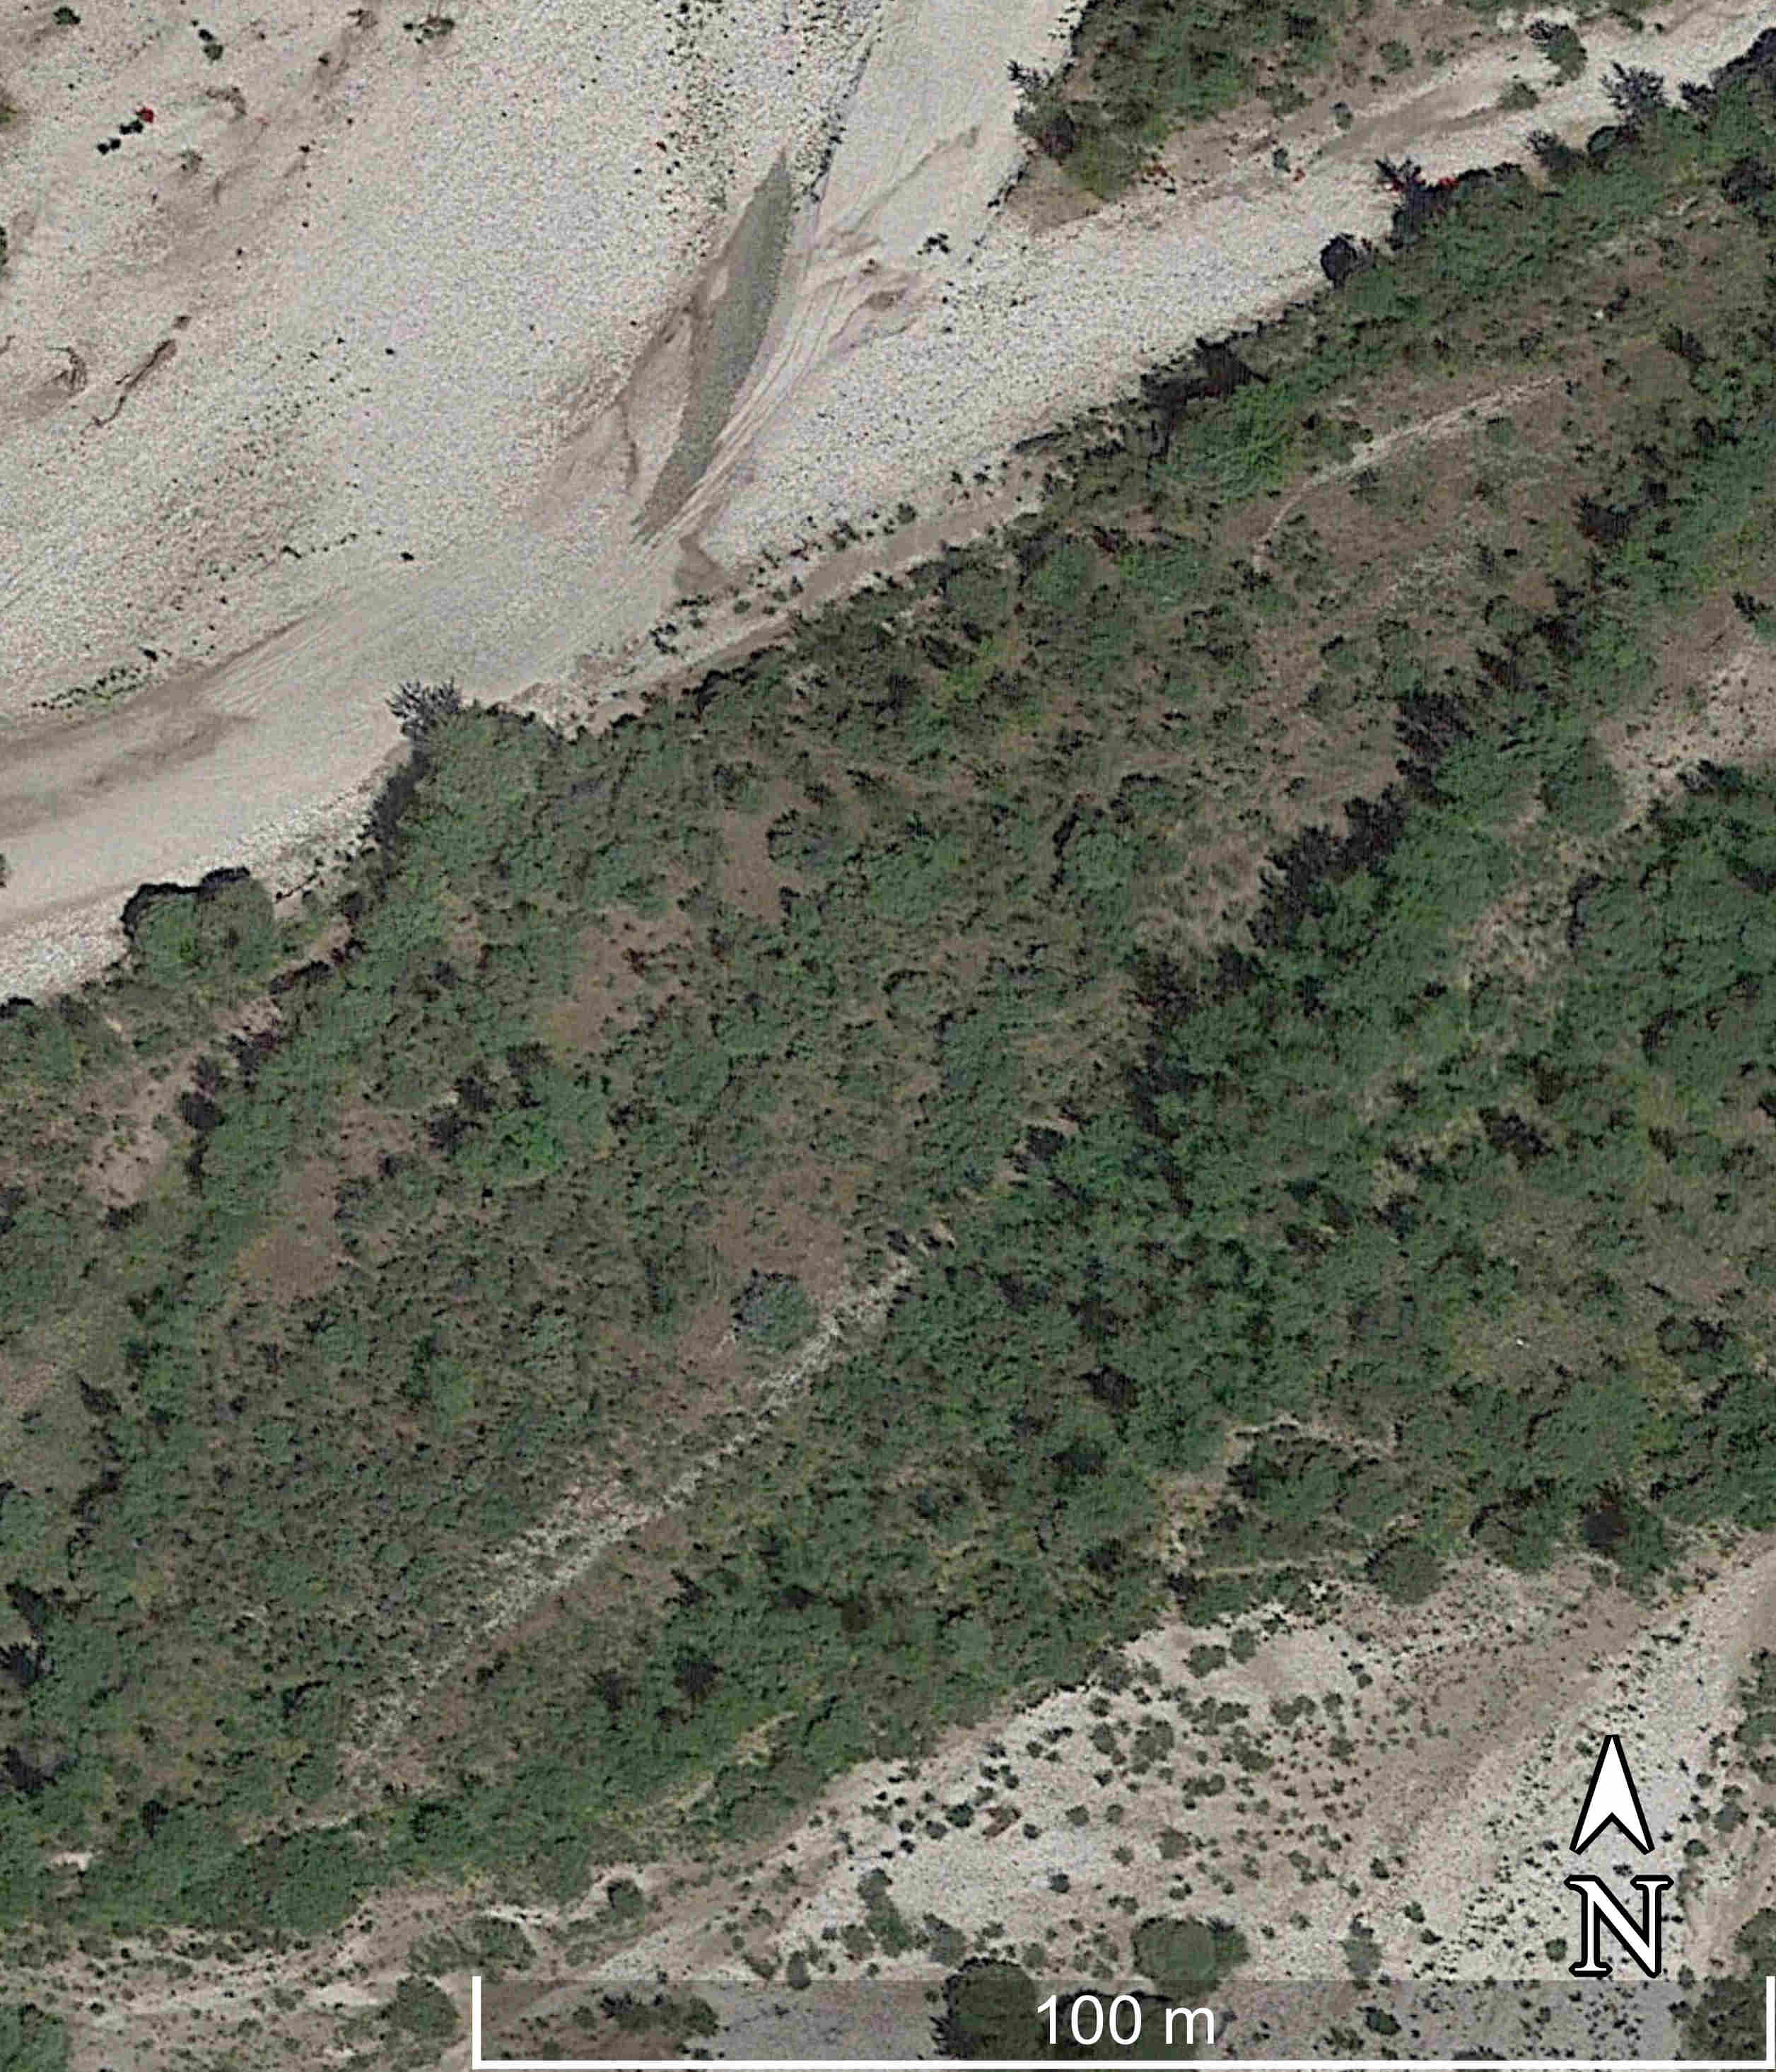
\includegraphics[width=\textwidth]{files/esempio_isola_sat_1.jpg}
		\caption{immagine da Google Earth di un isola in alveo.}
		\label{fig:esempio-isola-sat-1}
	\end{subfigure}
	\quad
	\begin{subfigure}[b]{0.57\textwidth}
		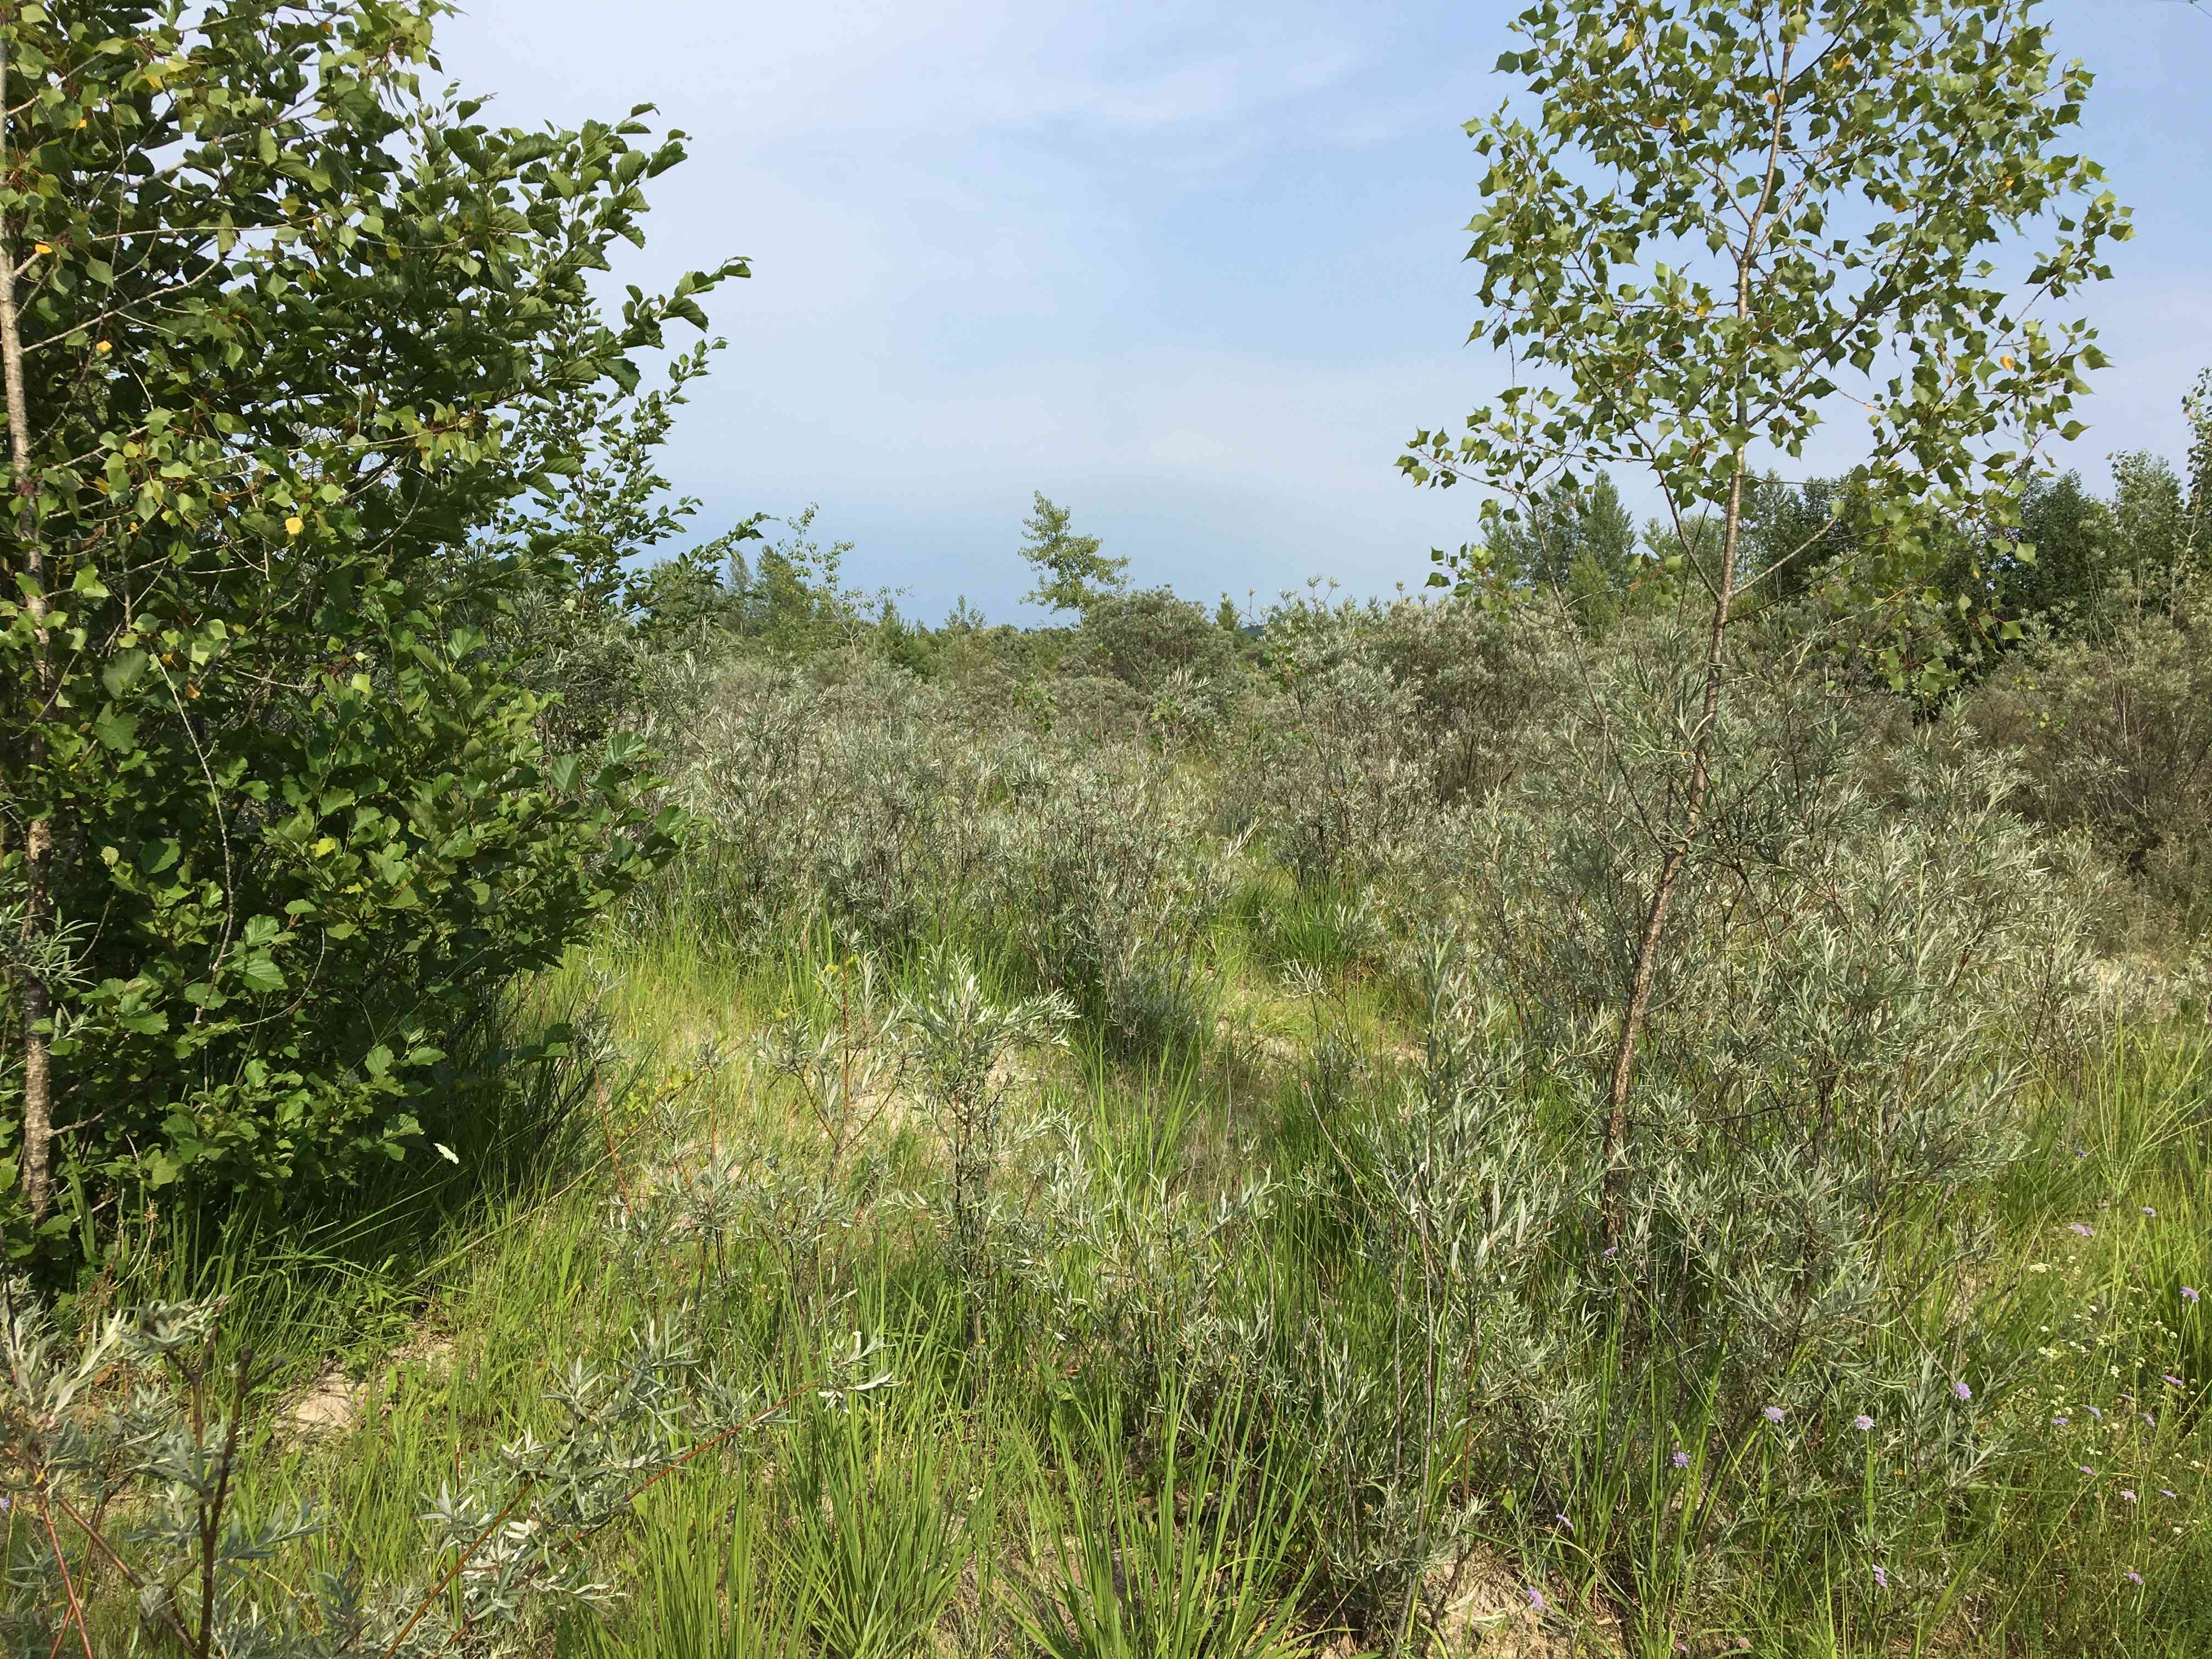
\includegraphics[width=\textwidth]{files/esempio_isola_1.jpg}
		\caption{foto di un isola molto vegetata presente nell'alveo del fiume.
		Foto dell'autore.}
		\label{fig:esempio-isola-1}
	\end{subfigure}
	\caption[immagine e foto di isole fluviali]{immagine e foto di isole fluviali; si noti la forte presenza di salici (\emph{Salix spp.}) e di pioppi (\emph{Populus spp.}); il luogo della foto è prossimo a quello dell'immagine.}
\end{figure}

\begin{figure}
	\centering
	\begin{subfigure}[b]{0.52\textwidth}
		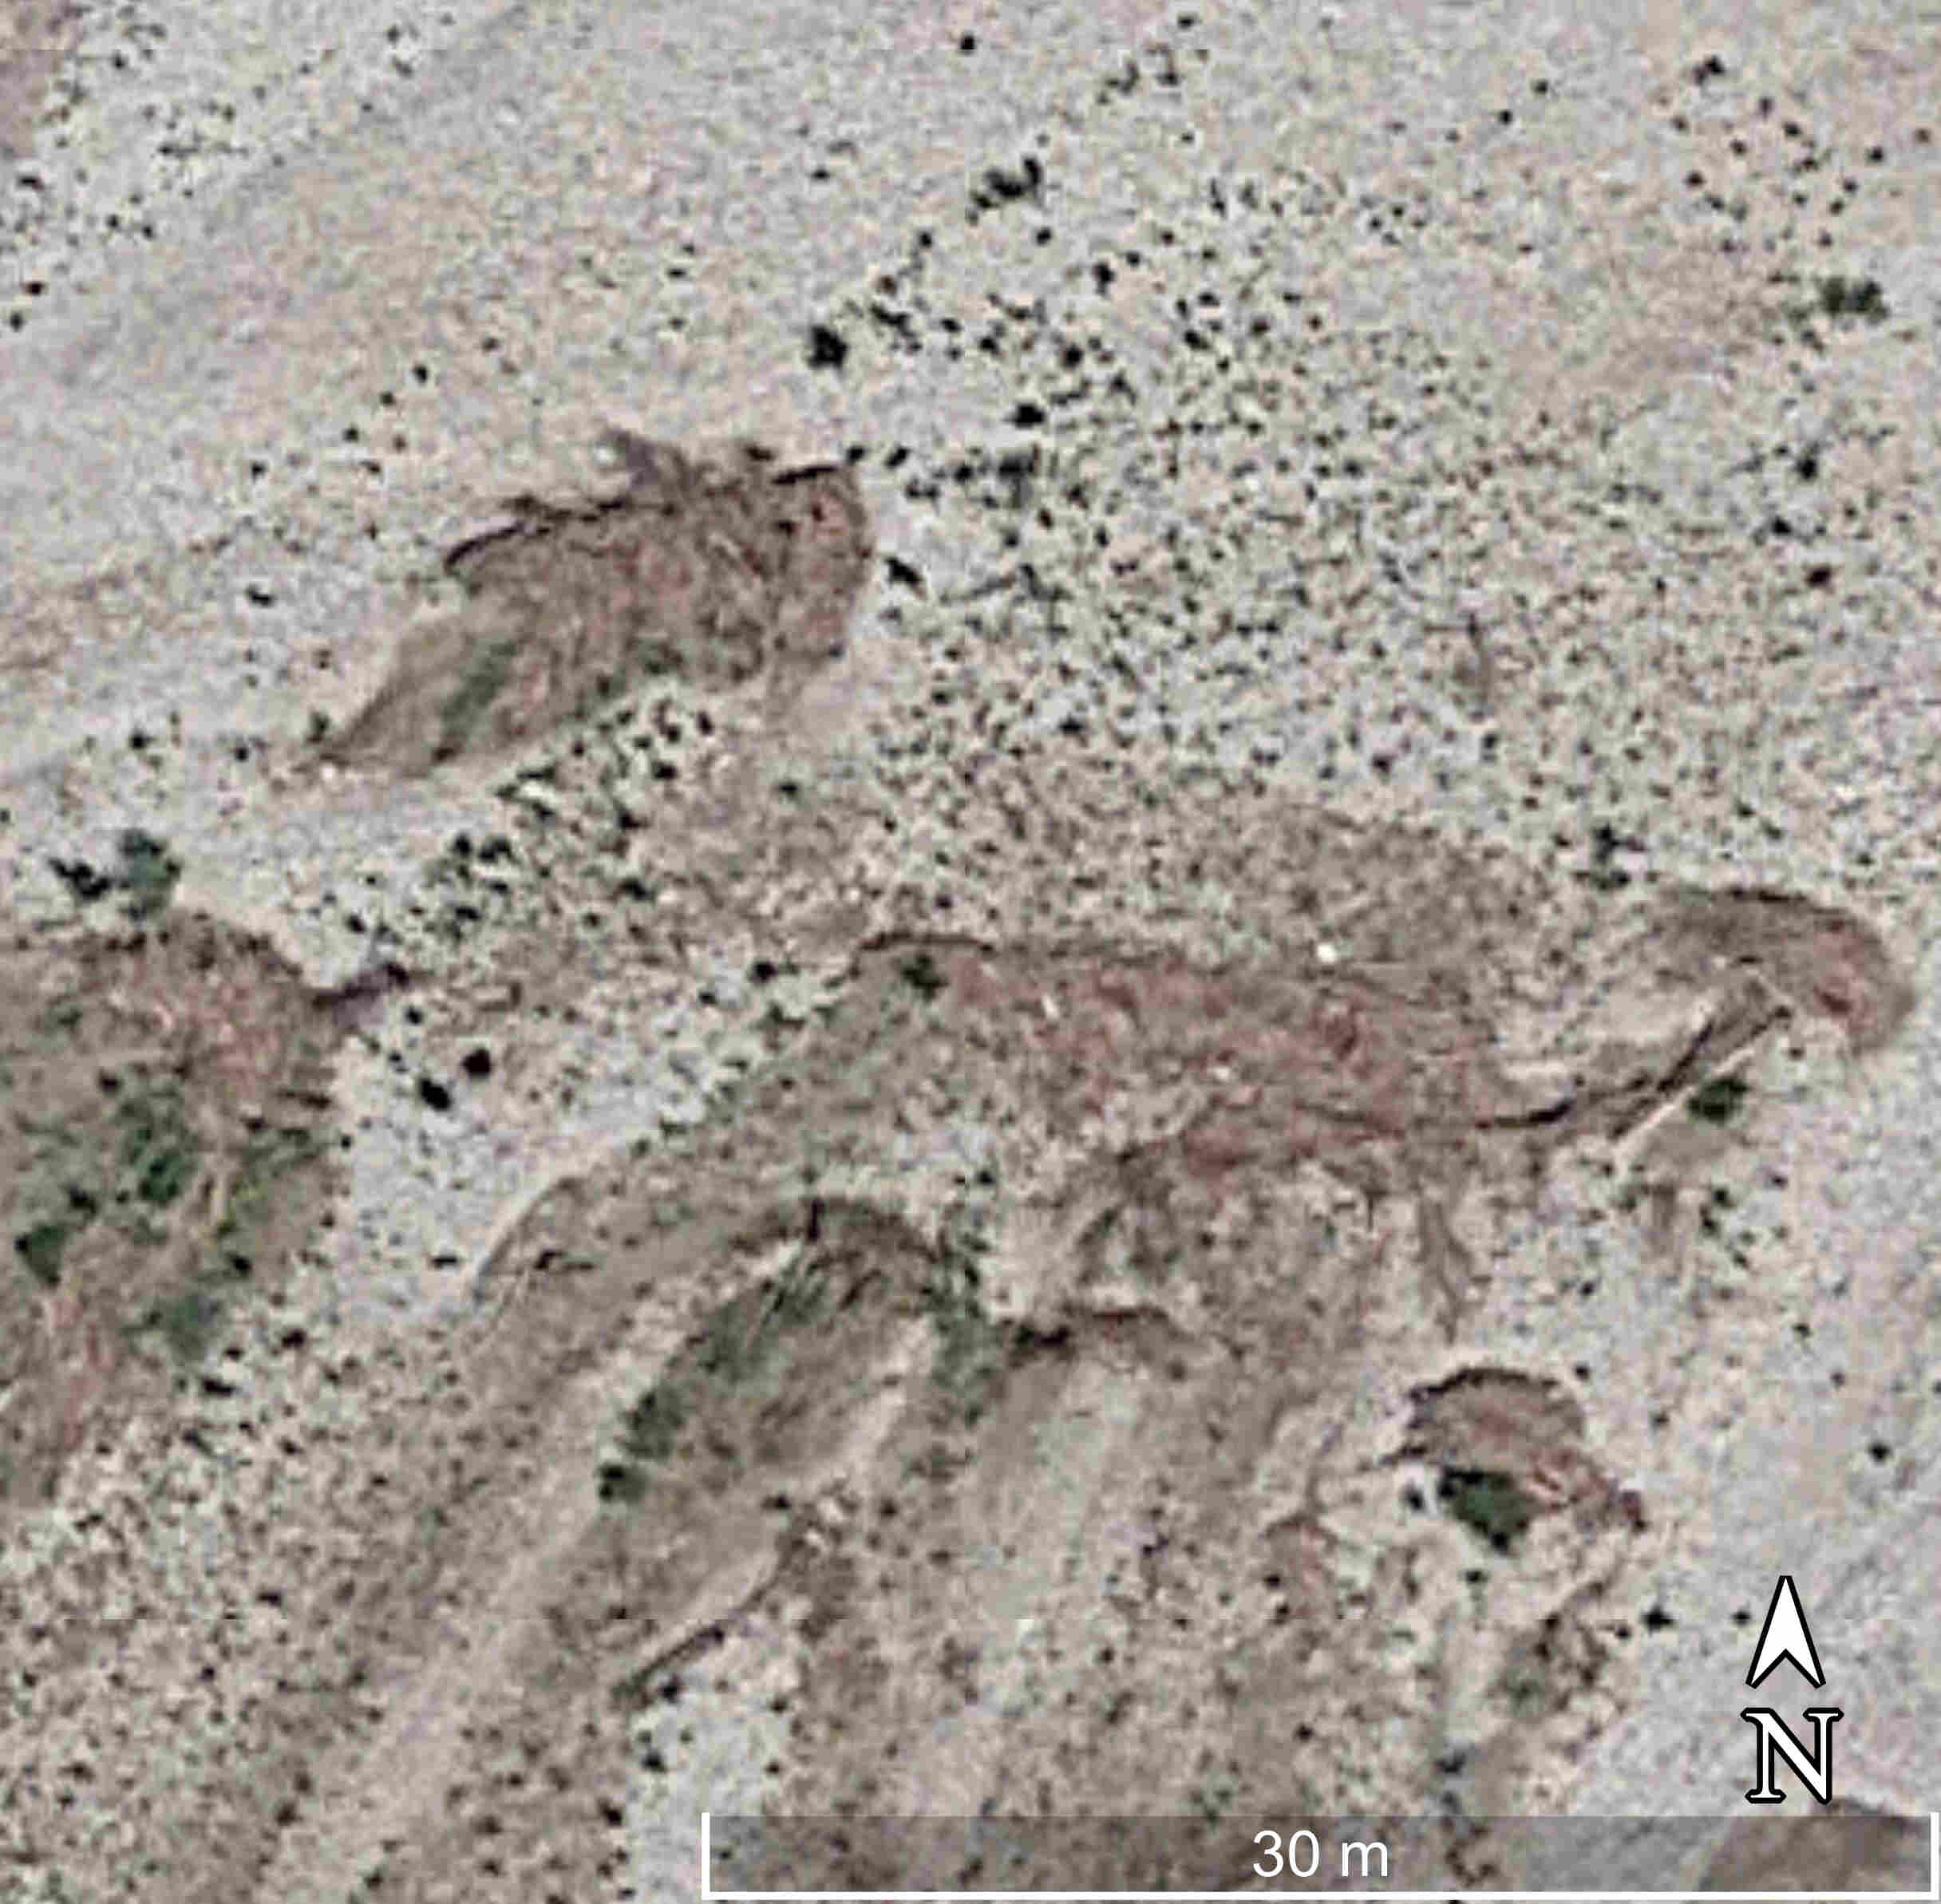
\includegraphics[width=\textwidth]{files/esempio_accumulo_sat_1.jpg}
		\caption{immagine da Google Earth di accumuli di legno e tronchi in alveo (in marrone chiaro).}
		\label{fig:esempio-accumulo-sat-1}
	\end{subfigure}
	\quad
	\begin{subfigure}[b]{0.44\textwidth}
		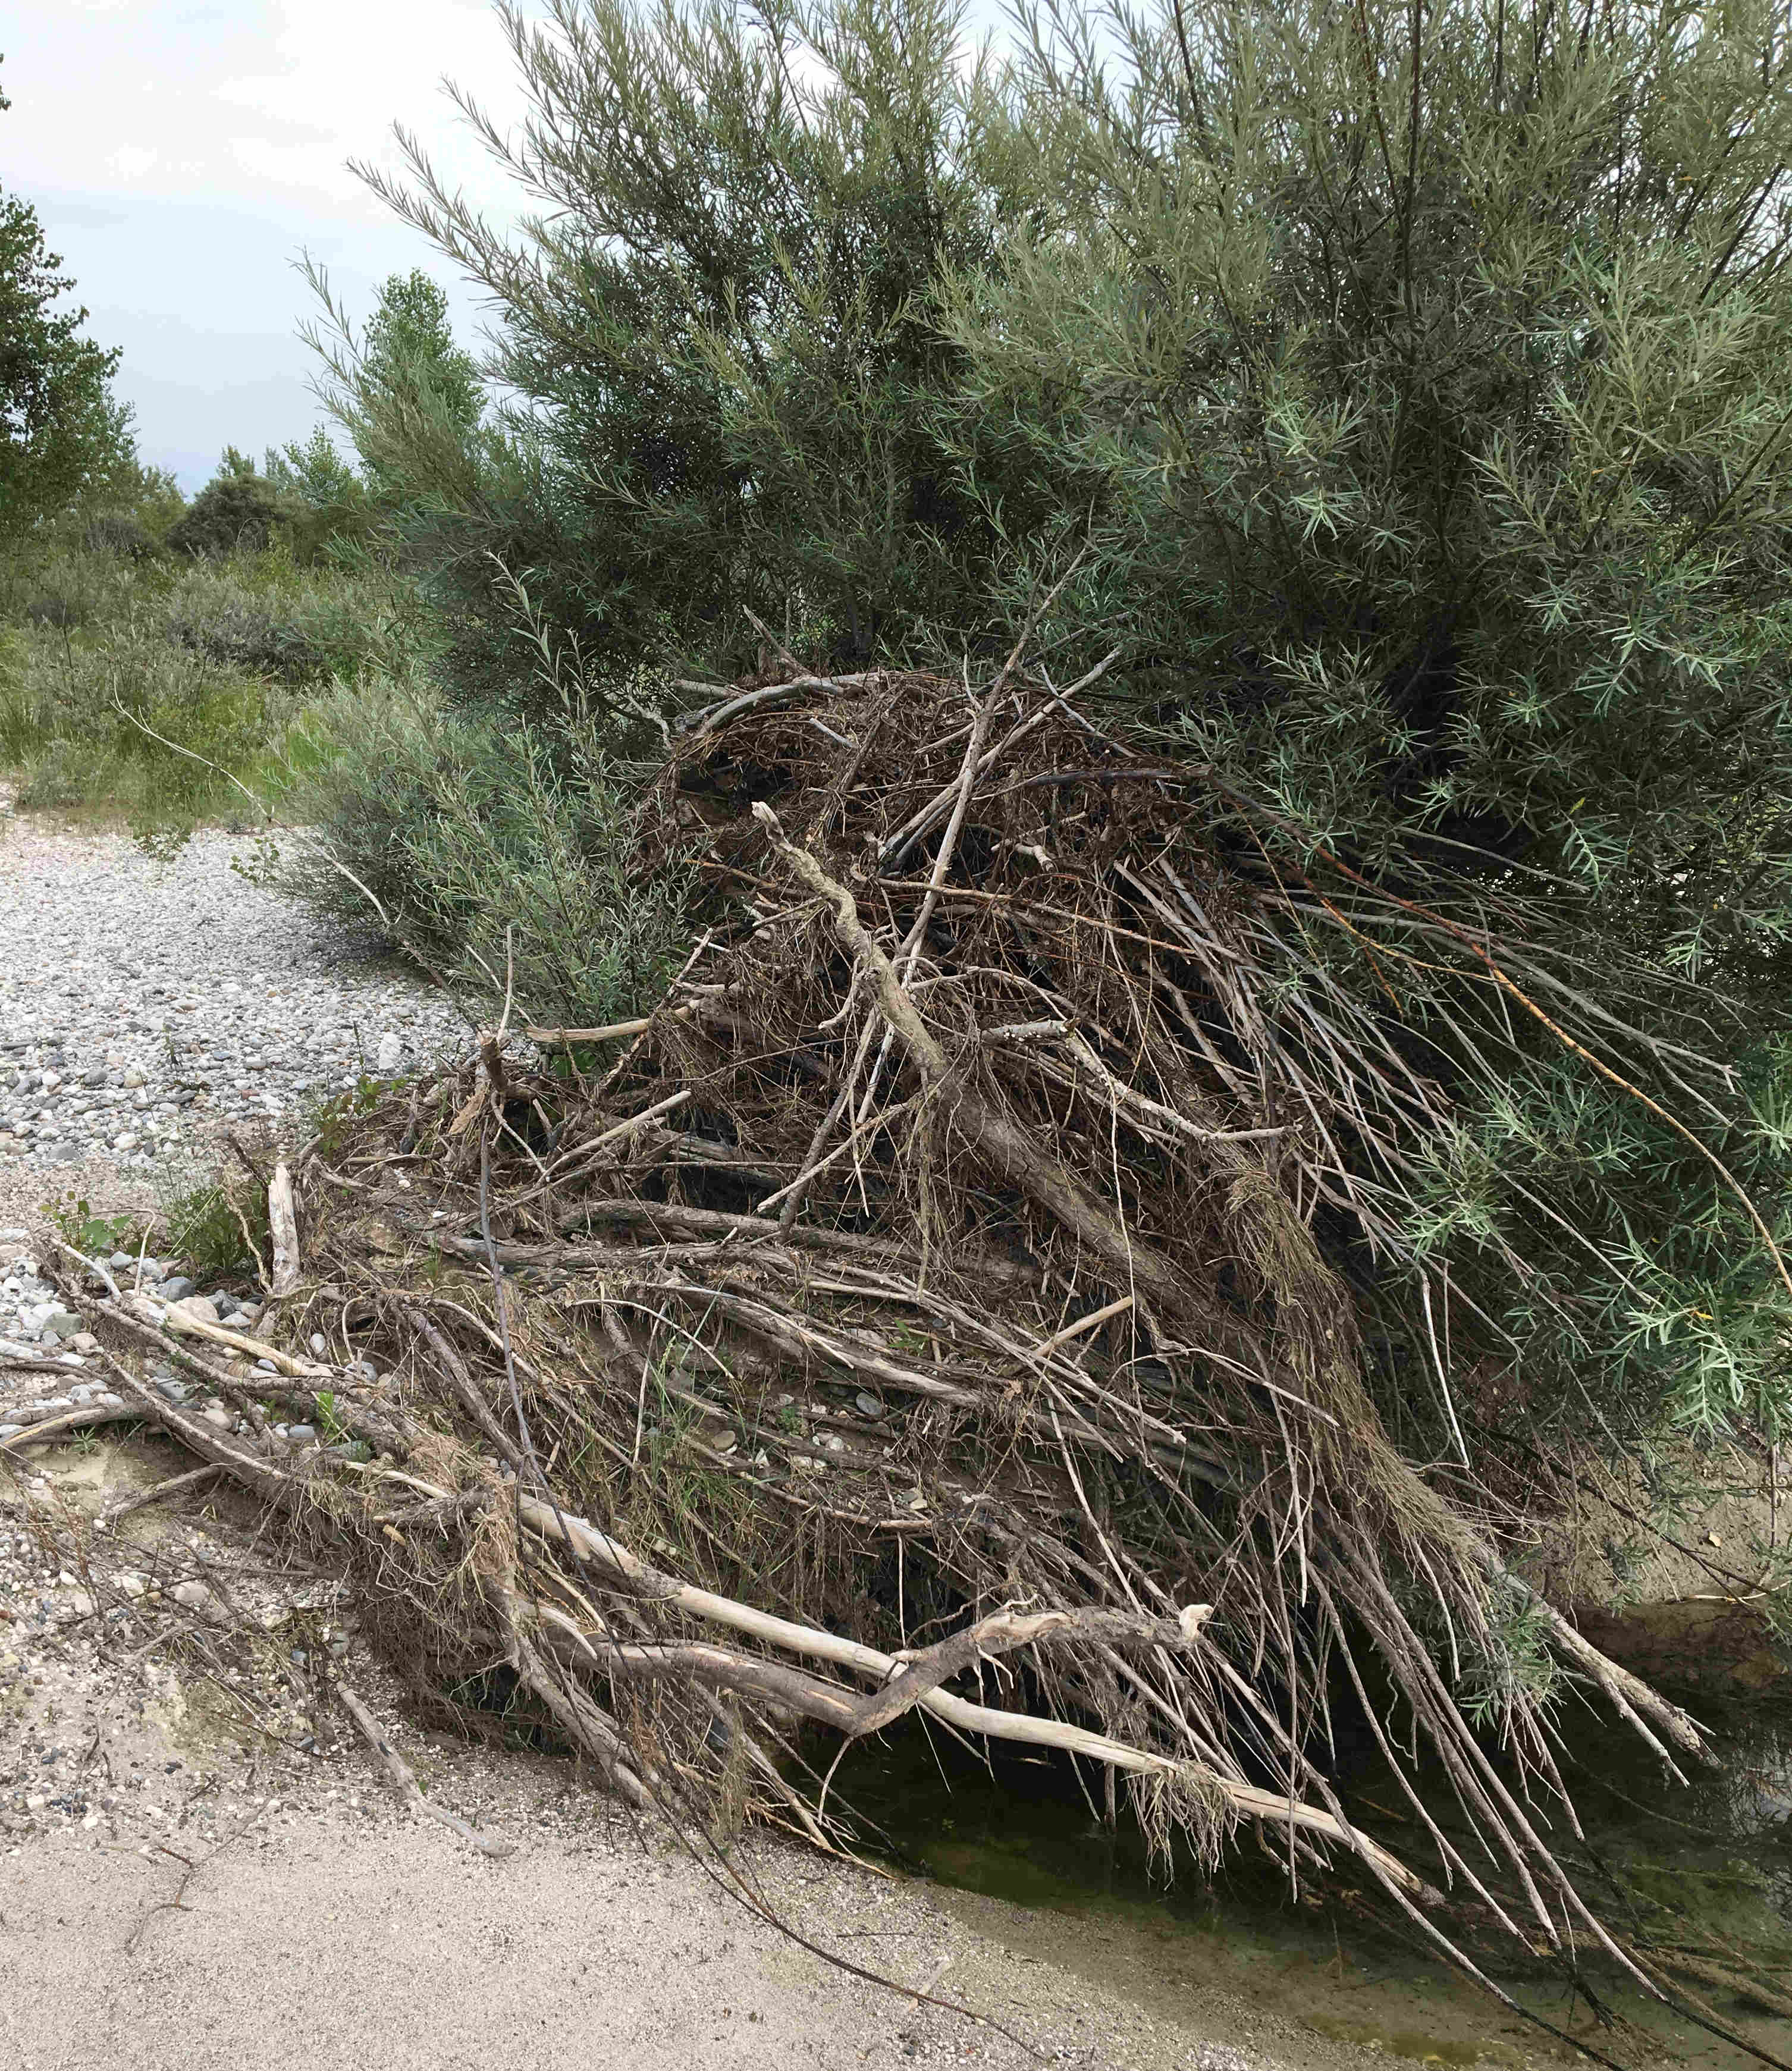
\includegraphics[width=\textwidth]{files/esempio_accumulo_1.jpg}
		\caption{foto di un accumulo di tronchi sopra una pianta di salice.
		Foto dell'autore.}
		\label{fig:esempio-accumulo-1}
	\end{subfigure}
	\caption[immagine e foto di accumuli legnosi]{immagine e foto di accumuli legnosi. Il luogo della foto non corrisponde a quello dell'immagine.}
\end{figure}

Con i dati di piovosità media mensile e di temperatura media mensile si cercano correlazioni con l'espansione della vegetazione che si osserva negli anni.
Dalla quantificazione dell'erosione della vegetazione dovuta alle piene, della quantità di legno in alveo e di un tasso di crescita della vegetazione si tenta di costruire un bilancio di materia vegetale a scala di evento di piena.
Inoltre si trovano valori soglia del livello del pelo libero per l'erosione della vegetazione.


\section{Bande}
Gli strumenti di acquisizione di immagini aeree e satellitari sono sensibili a determinate lunghezze d'onda della radiazione elettromagnetica (\vref{graph:el-mag-radiation}), cioè sono in grado di registrarne solo alcune porzioni (bande). 
L'occhio umano può distinguere solo le bande del visibile, mentre i sensori artificiali possono acquisire altre bande della radiazione. 
%
\begin{figure}
	\centering
	\tikzsetnextfilename{electromagnetic_radiation}
\begin{tikzpicture}[fill between/on layer={axis grid}]
	\begin{axis}[
		xlabel={Lunghezza d'onda},
		xticklabel style = {font=\tiny,yshift=0.2ex},
		xmin=10^-5,
		xmax=10^9,
		x unit=\si{\micro\meter},
		xmode=log,
		ymin=0,
		ymax=1,
		height=3cm,
		width=\textwidth,%12.2cm,
		yticklabels={},
		ytick=\empty,
		legend cell align=left,
		legend style={
			at={(0.5,-0.8)},%(0.85,-0.77)},
			anchor=north,
			legend columns=4,
			}
	]
	\addplot[draw=none, name path=start, forget plot] coordinates{(10^-5,0)(10^-5,1)};
	\addplot[draw=none, name path=gamma, forget plot] coordinates{(10^-3,0)(10^-3,1)};
	\addplot[draw=none, name path=xrays, forget plot] coordinates{(10^-2,0)(10^-2,1)};
	\addplot[draw=none, name path=uv, forget plot] coordinates{(0.4,0)(0.4,1)};
	\addplot[draw=none, name path=visible, forget plot] coordinates{(0.7,0)(0.7,1)};
	\addplot[draw=none, name path=ir, forget plot] coordinates{(10^2.5,0)(10^2.5,1)};
	\addplot[draw=none, name path=microwave, forget plot] coordinates{(10^5,0)(10^5,1)};
	\addplot[draw=none, name path=radiowave, forget plot] coordinates{(10^9,0)(10^9,1)};
	\addplot[violet!20, area legend] fill between[of=start and gamma];
	\addlegendentry{Raggi $\gamma$}
	\addplot[violet!60, area legend] fill between[of=gamma and xrays];
	\addlegendentry{Raggi X}
	\addplot[violet, area legend] fill between[of=xrays and uv];
	\addlegendentry{Ultravioletti}
	\addplot[shading=visiblelight, area legend] fill between[of=uv and visible];
	\addlegendentry{Luce visibile}
	\addplot[red, area legend] fill between[of=visible and ir];
	\addlegendentry{Infrarosso}
	\addplot[Bittersweet, area legend] fill between[of=ir and microwave];
	\addlegendentry{Microonde}
	\addplot[Brown, area legend] fill between[of=microwave and radiowave];
	\addlegendentry{Onde radio}
	\end{axis}
\end{tikzpicture}

	\caption{radiazione elettromagnetica con le sue lunghezze d'onda.}
	\label{graph:el-mag-radiation}
\end{figure}
%
\\
Le immagini nel visibile sono solitamente suddivise nelle bande del Rosso, Verde e Blu (\emph{Red}, \emph{Green}, \emph{Blue}, R-G-B); ognuna indica la quantità di colore presente; la combinazione di queste quantità di colore restituisce l'immagine a colori. 
\\
Per poter osservare immagini con bande diverse dal visibile si sostituisce una o più bande R-G-B con le bande in questione. 
Ad esempio, è possibile sostituire la banda del Rosso con quella dell'Infrarosso (IR): la quantità di colore del Rosso sarà rimpiazzata dalla quantità di colore dell'Infrarosso. 
Il risultato sarà un'immagine riconoscibile dall'occhio umano, ma in falsi colori (\vref{fig:confronto-bande-intro}).
%
\begin{figure}
	\centering
	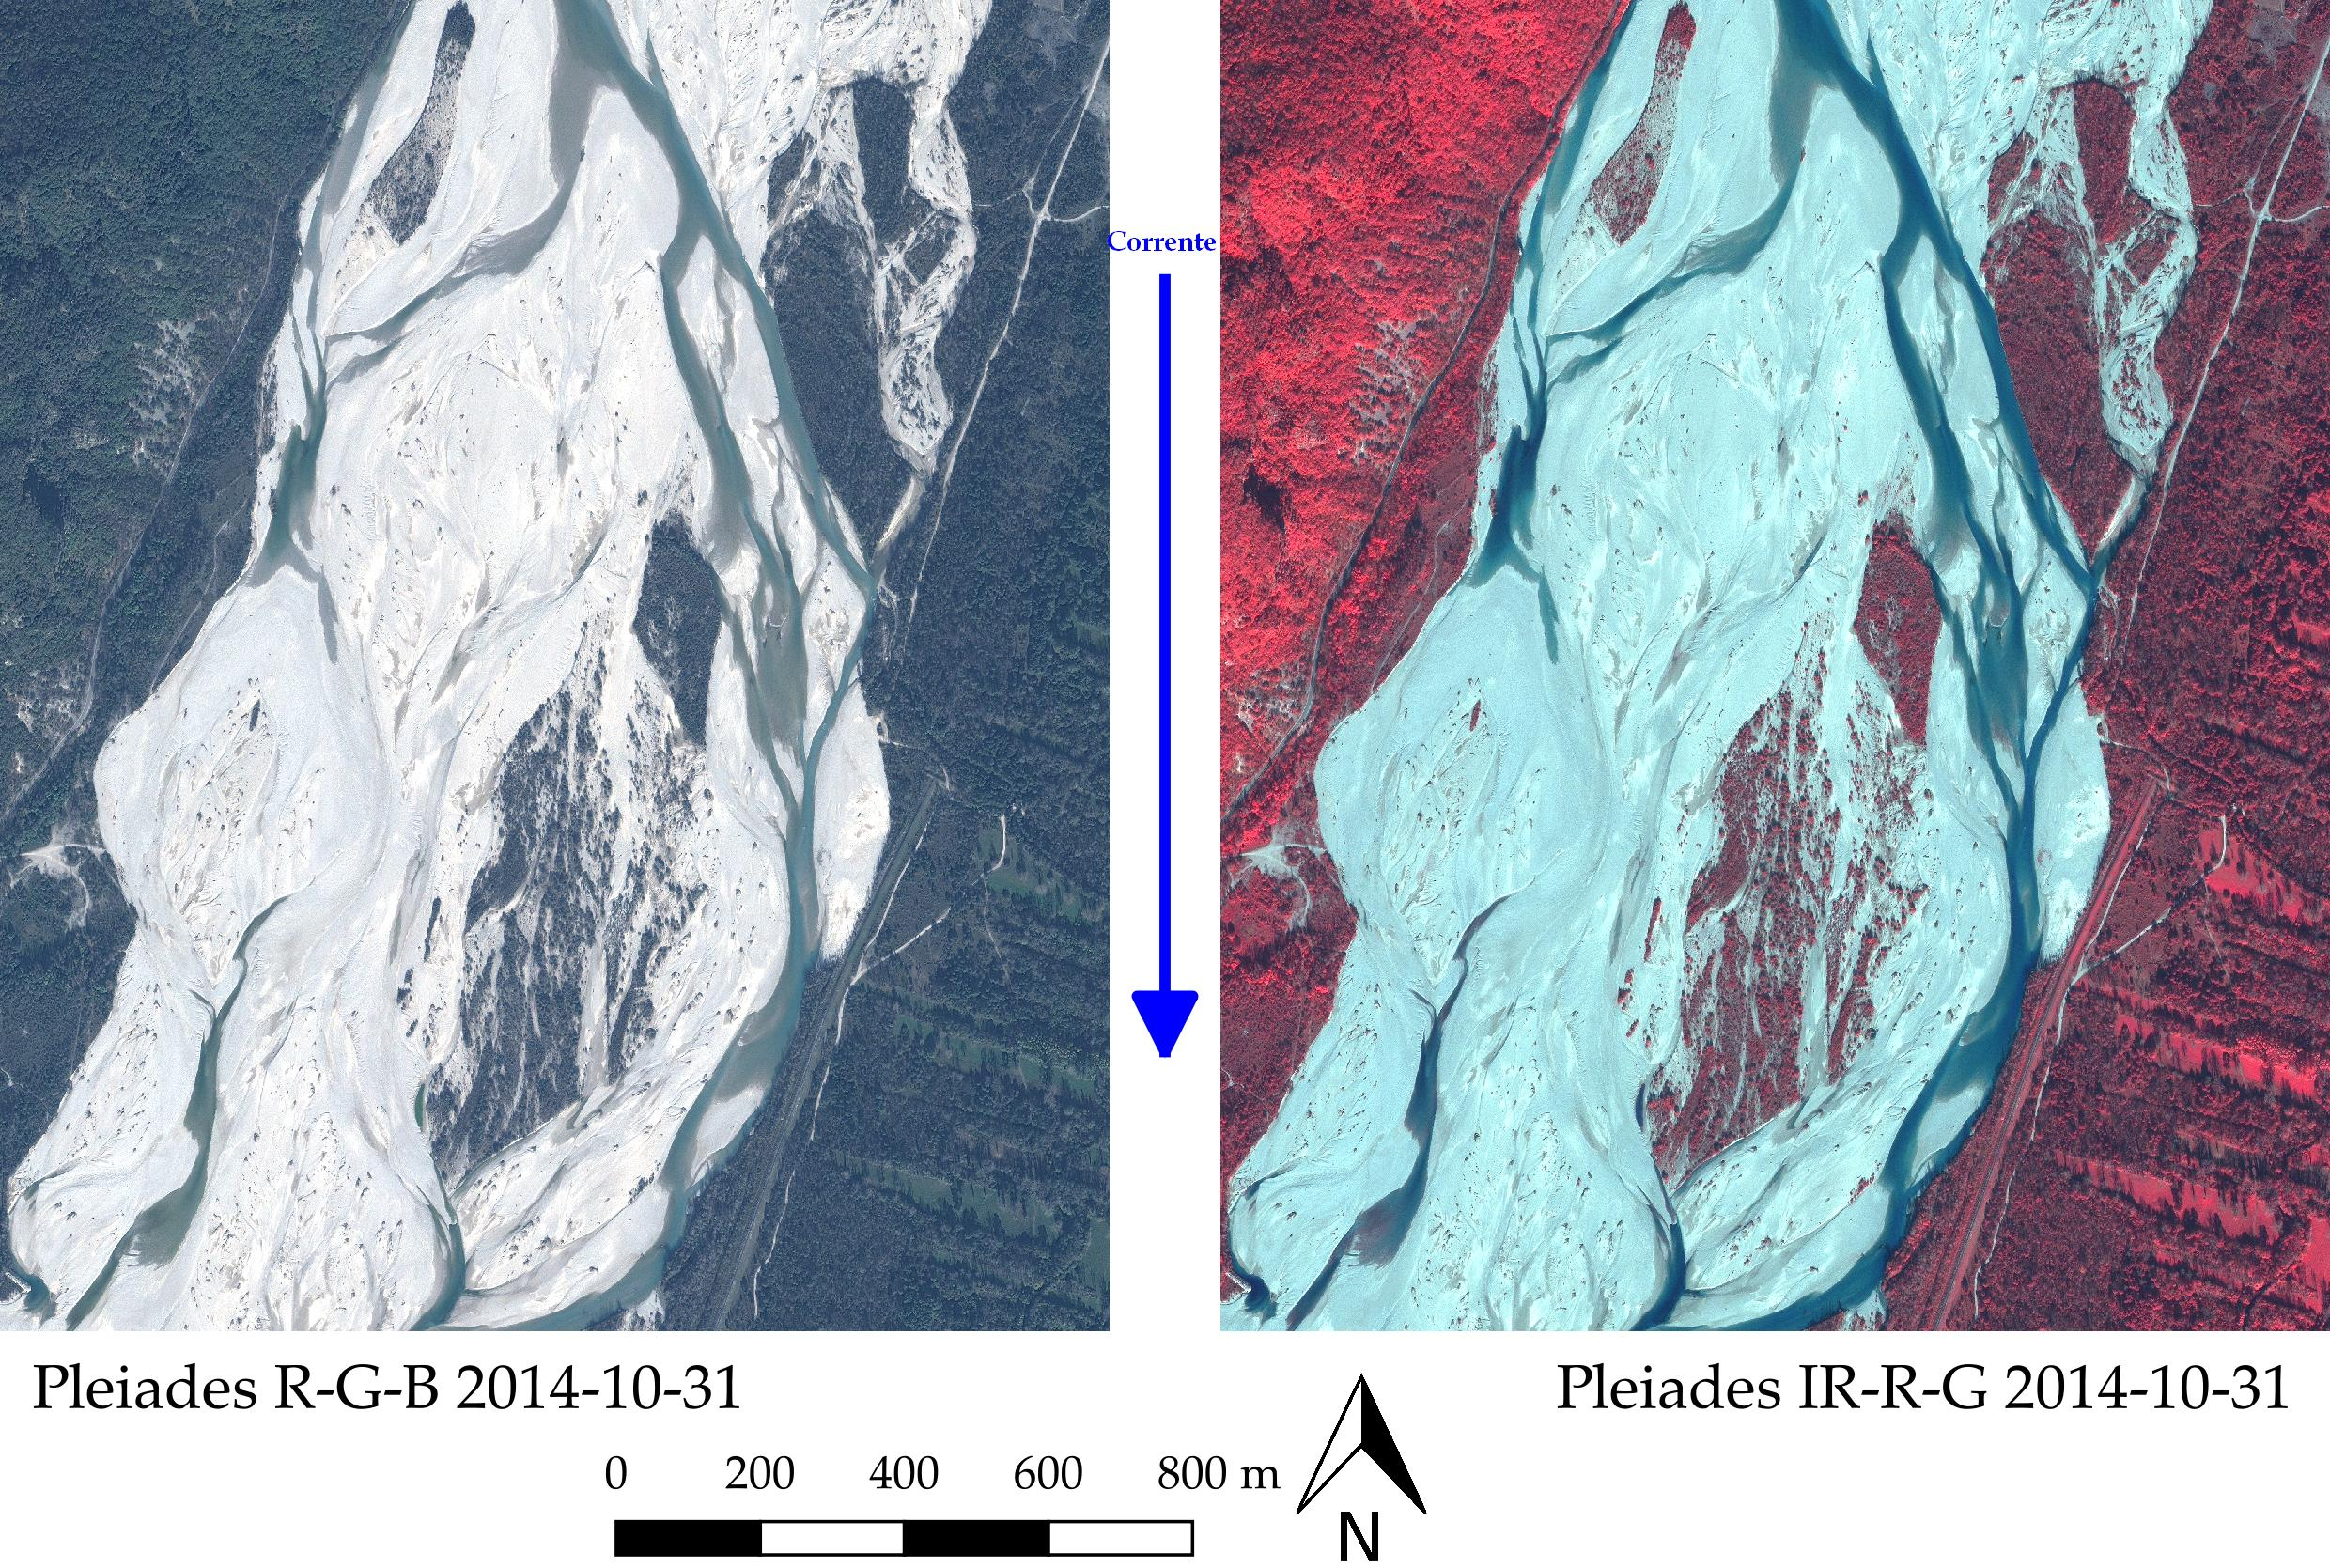
\includegraphics[width=\textwidth]{files/confronto_bande_intro.jpeg}
	\caption[confronto immagini R-G-B e IR-R-G]{confronto di un'immagine in veri colori (R-G-B, a sinistra) con una in falsi colori (IR-G-B, a destra); quest'ultima evidenza la presenza di vegetazione viva rispetto alla ghiaia in alveo e all'acqua nei canali.}
	\label{fig:confronto-bande-intro}
\end{figure} 
%
\\
Questo procedimento serve per distinguere più facilmente degli elementi e degli oggetti presenti nelle immagini; per esempio la vegetazione viva riflette particolarmente la banda dell'Infrarosso più vicina al Rosso.




\section{Inquadramento dell'area di studio}
Il Fiume Tagliamento, situato nel Nord-Est italiano, è uno dei pochi fiumi alpini allo stato quasi naturale. 
Il suo bacino idrografico, ampio circa~\SI{2900}{\kilo\m\tothe{2}}, si estende tra le province di Udine, Pordenone e Venezia.
Il suo corso di circa~\SI{170}{\kilo\m} presenta morfologia intrecciata (\emph{braided}) nelle parti montane e planiziali; verso valle il fiume si restringe assumendo prima una forma transizionale monocursale nei pressi di Madrisio, infine meandriforme a Latisana.
\\
Il tratto studiato è quello intrecciato multicanale compreso tra Tolmezzo e Madrisio (\vref{fig:overview,fig:overview-gearth}).
%
\begin{figure}
	\centering
	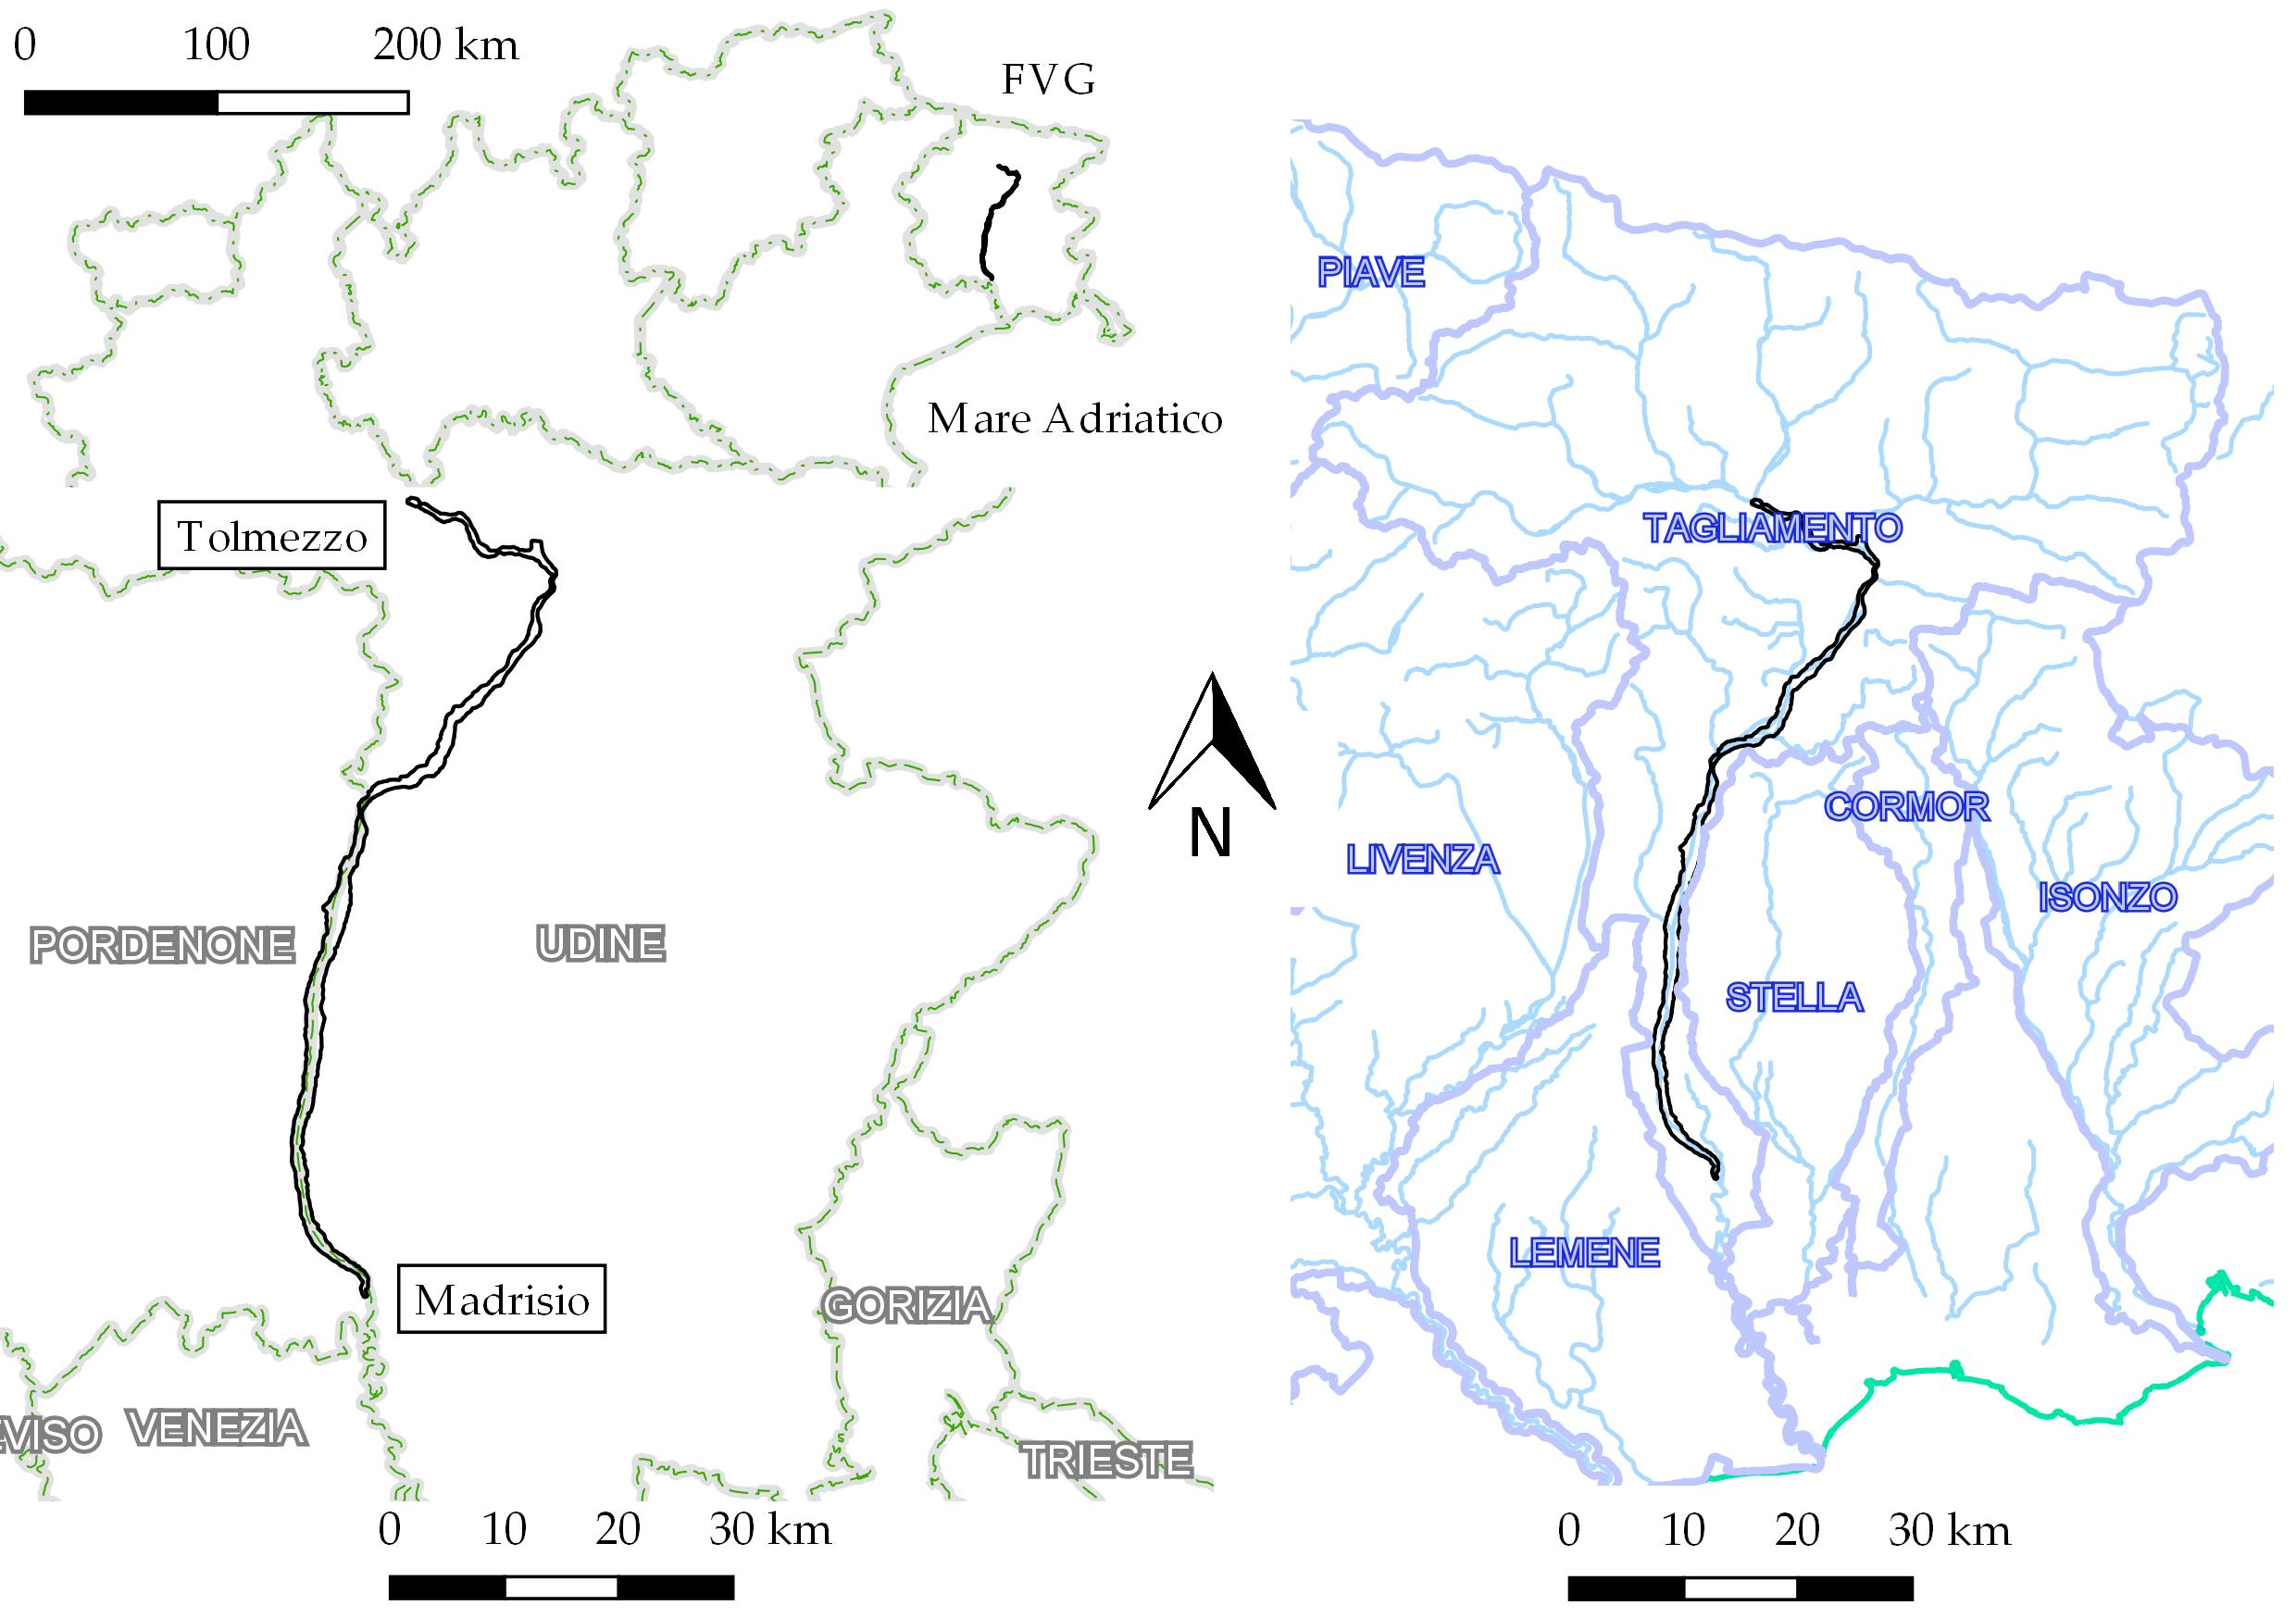
\includegraphics[width=\textwidth]{files/overview.jpeg}
	\caption[inquadramento dell'area di studio]
		{inquadramento dell'area di studio (poligono nero); a sinistra è mostrata l'Italia settentrionale (in alto) e un ingrandimento delle province e degli estremi dell'area di studio (in basso); a destra si vede il bacino idrografico del Tagliamento e di altri fiumi nelle vicinanze (in blu), il reticolo idrografico (in azzurro) e la linea di costa (in verde acqua).}
	\label{fig:overview}
\end{figure}
%
\begin{figure}
	\centering
	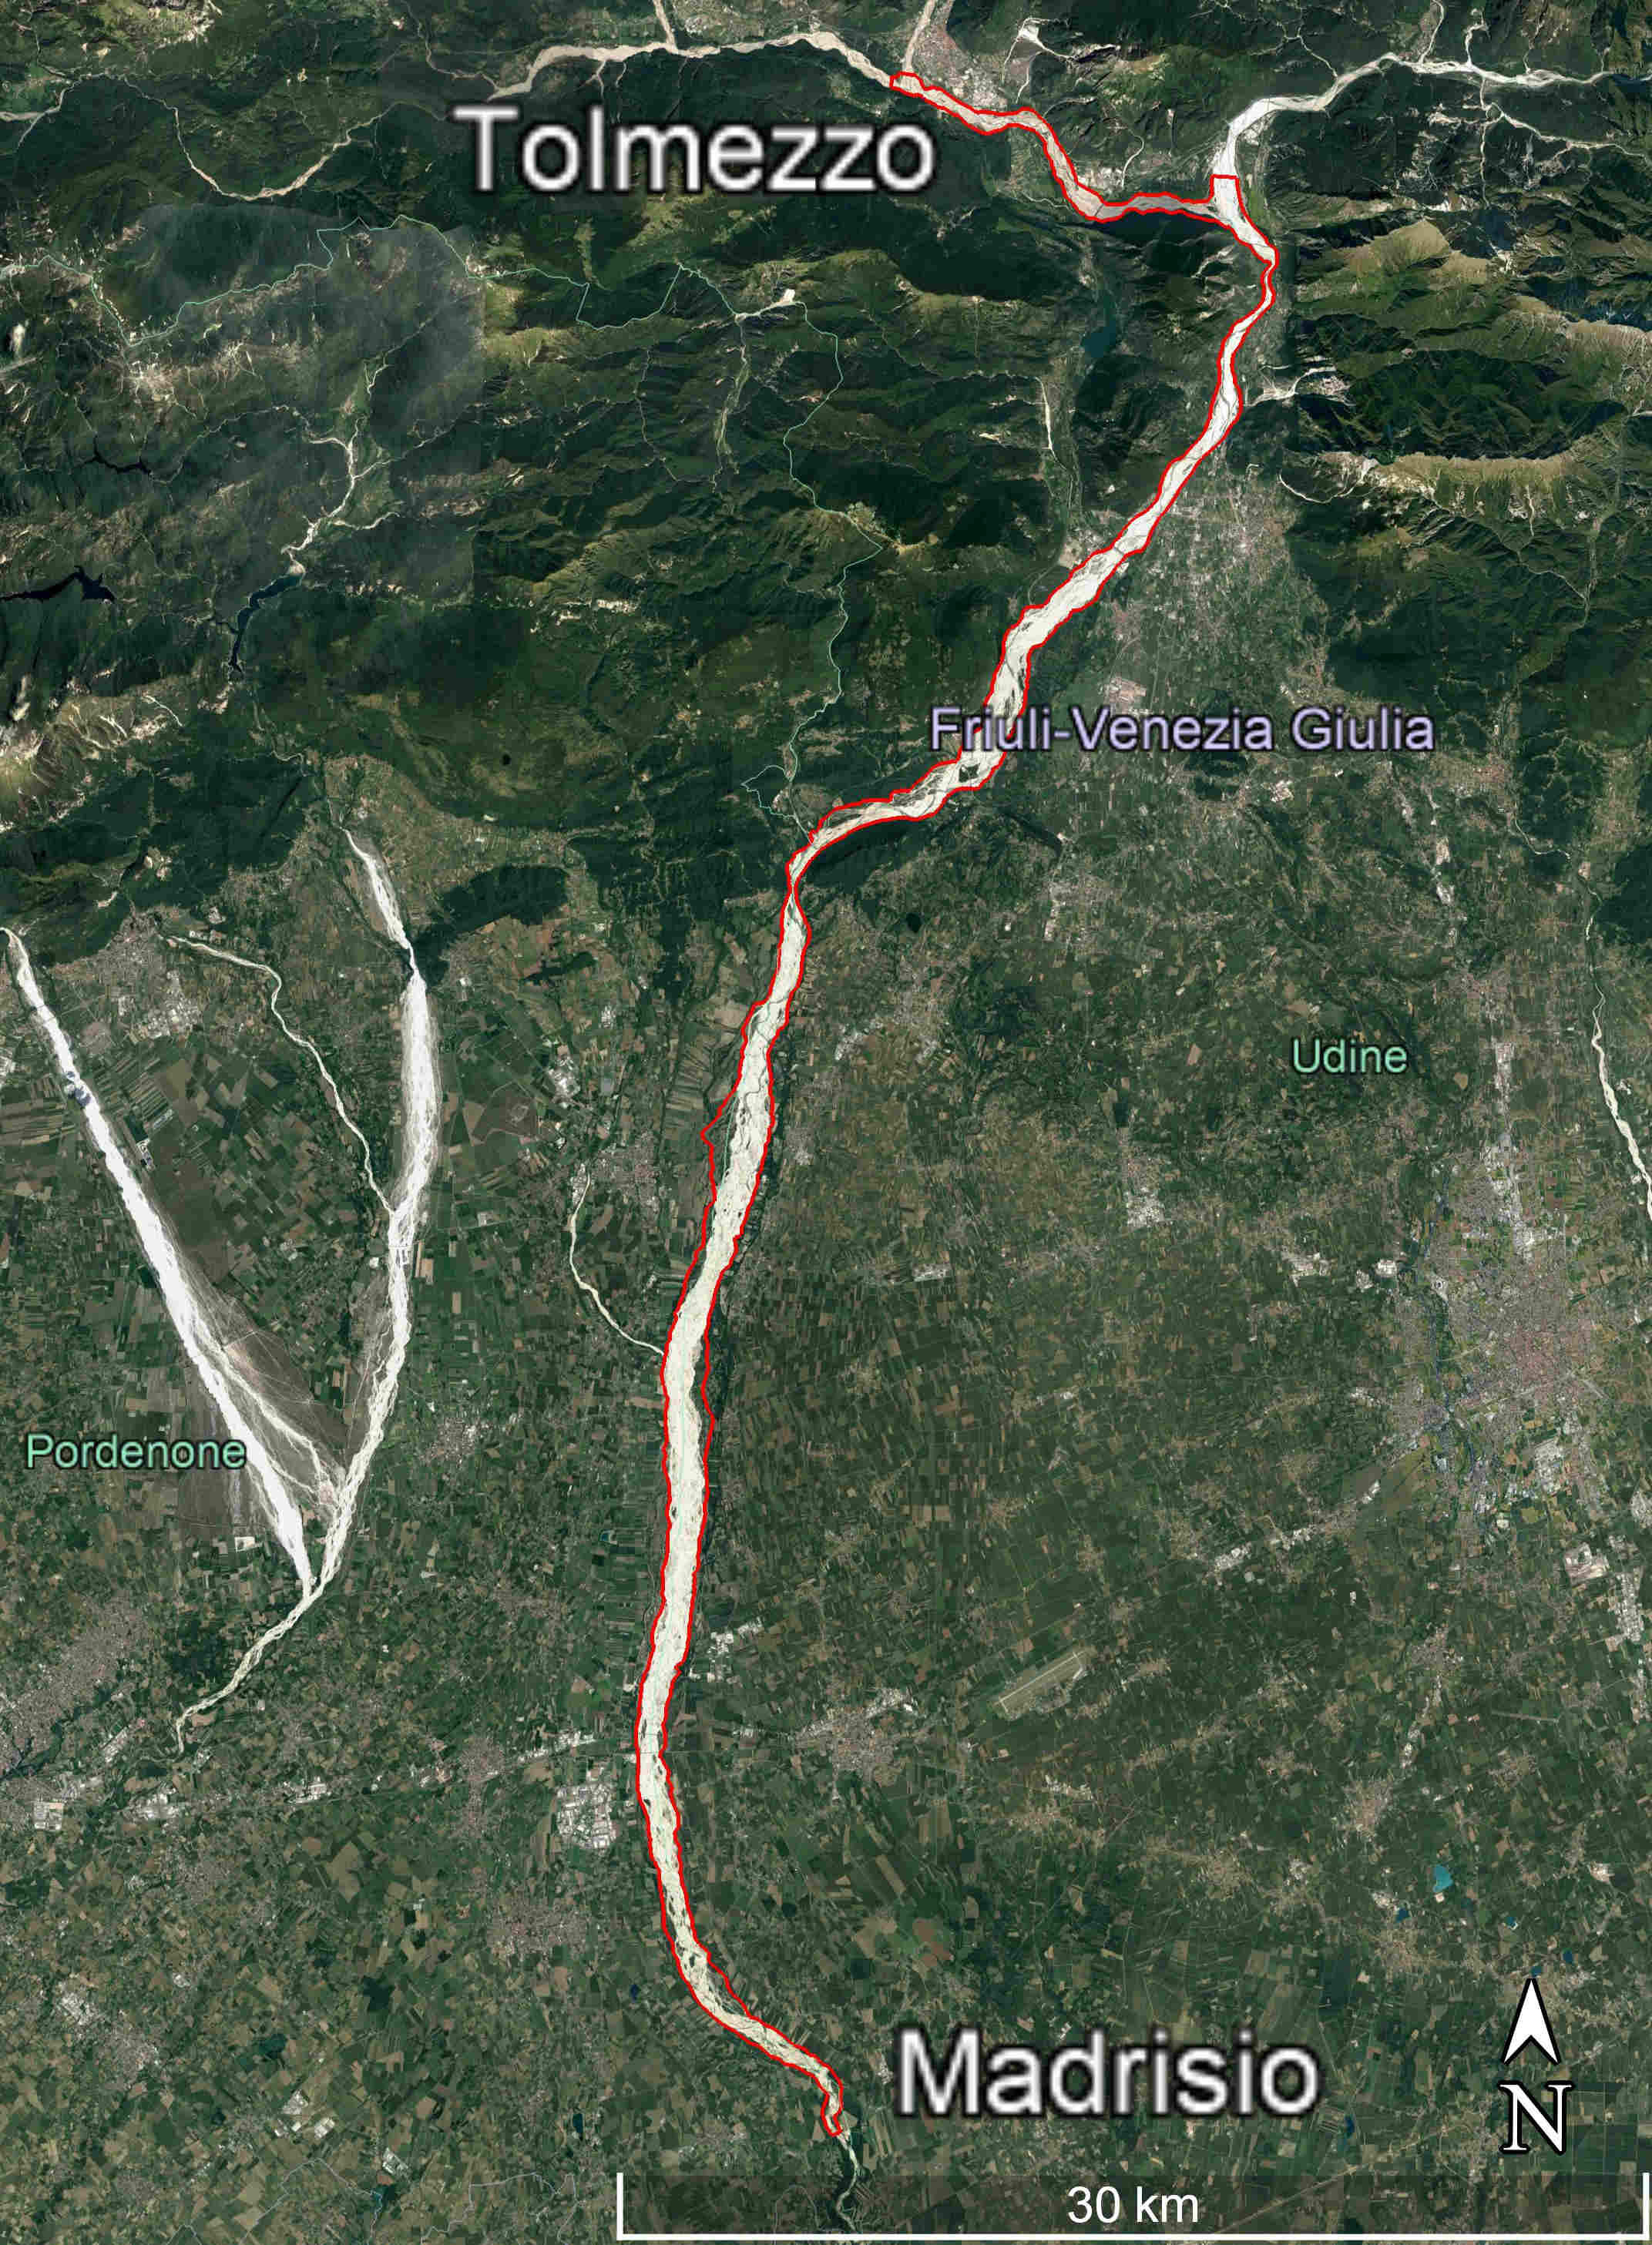
\includegraphics[width=.7\textwidth]{files/overview_gearth.jpg}
	\caption[inquadramento su Google Earth dell'area di studio]{inquadramento su Google Earth dell'area di studio (contornata in rosso).}
	\label{fig:overview-gearth}
\end{figure}



\section{Convenzioni}
Le seguenti convenzioni saranno utilizzate nella presente tesi:
\begin{description}
	\item[Mappe] riportate secondo WGS84/UTM~32N (EPSG:~32633);
	\item[Formato delle date] AAAA-MM-GG;
	\item[Citazioni] sono nel formato Autore/i-Anno, racchiuse tra parentesi quadre;
	\item[Web link] sono riportati in note a piè pagina;
	\item[Termini in lingua straniera] sono in corsivo;
	\item[Glossario] presente nel materiale finale;
	%
\end{description}



\section{Materiali}
% materiali
Sono state considerate le bande del \emph{Near-InfraRed}~(NIR) e del \emph{Red}~(R) nelle immagini satellitari multibande provenienti dalle seguenti missioni:
%
\begin{itemize}
	\item satellite Terra, sensore ASTER Livello~1T (ottenuti in data~21~luglio~2018 \squarecite{data:ASTER});  
		\\
		NIR (Banda~3N)~\SIrange[range-phrase={-}]{0.78}{0.86}{\nano\m}, R (Banda~2)~\SIrange[range-phrase={-}]{0.63}{0.69}{\micro\m};
	\item costellazione Pleiades (\href{https://pleiades.cnes.fr/en/PLEIADES/index.htm}{Centre National d'Etudes Spatiales}\footnote{\texttt{https://pleiades.cnes.fr/en/PLEIADES/index.htm}}); 
		\\
		NIR~\SIrange[range-phrase={-}]{0.74}{0.94}{\micro\m}, R~\SIrange[range-phrase={-}]{0.59}{0.71}{\micro\m};
	\item satellite Sentinel2A, sensore~MSI Livello~1C (ottenuti in data 21~luglio 2018 tramite la API del \href{http://scihub.copernicus.eu/}{Copernicus Open Access Hub}\footnote{\texttt{http://scihub.copernicus.eu/}});
		\\
		NIR (Banda~8)~\SIrange[range-phrase={-}]{0.763}{0.908}{\micro\m}, R (Banda~4)~\SIrange[range-phrase={-}]{0.645}{0.683}{\micro\m}.
\end{itemize}
%

Le ortofoto dell'estate~2011 provengono dal \href{http://www.pcn.minambiente.it/mattm/}{Portale Cartografico Nazionale del Ministero dell'Ambiente e della tutela del territorio e del mare}\footnote{\texttt{http://www.pcn.minambiente.it/mattm/}};
le ortofoto del~2013 sono state effettuate su commissione; 
%
%
le ortofoto del~2017 sono state ottenute da \href{https://www.google.com/earth/}{Google Earth}\footnote{\texttt{https://www.google.com/earth/}}.
\\
I dati idrometrici sono stati forniti dalla \href{http://www.protezionecivile.fvg.it/it/rete-idrometeorologica}{rete idrometeorologica della Protezione Civile della Regione Autonoma Friuli Venezia Giulia}\footnote{\texttt{http://www.protezionecivile.fvg.it/it/rete-idrometeorologica}}.
\\
I grafici in \vref{graph:livelli-orto-sat} mostrano rispettivamente i livelli idrometrici registrati presso l'idrometro di Villuzza, corrispondente al ponte di Pinzano, e le date di cui si dispongono ortofoto e immagini satellitari (ASTER, Pleiades, Sentinel2, Google~Earth). 
Nel secondo grafico sono riportati solamente i livelli maggiori di~\SI{2}{\m} in quanto livelli superiori a tale soglia iniziano ad avere effetti di disturbo sulla vegetazione \squarecite{Bertoldi:2009-2m}.
La \vref{tab:date-orto-sat} mostra le date e la risoluzione delle immagini utilizzate nell'analisi.
%%
\begin{figure}[p]
	\centering
	\begin{tikzpicture}
	%\begin{groupplot}
	\begin{axis}[
		%name = orto-sat,
		axis y line* = right,
		axis x line* = top,
		%height = .3\textwidth,
		width = \textwidth,
		date coordinates in = x,
		%symbolic y coords = {ASTER,PLEIADES,SENTINEL2,G-EARTH},
		xticklabel = {\year-\month-\day},
		xtick = data,
		ytick = data,
		xticklabel style = {
			rotate = 90,
			anchor = near xticklabel
		},
		enlarge x limits = 0.05,
		enlarge y limits = 0.01,
		ylabel = {Fonte},
		ymax = 3.6,
		ymin = -0.1,
		grid = none,
		only marks,
		]
		\addplot table [x=data, y=numero] {graphics/data/data-orto-sat.txt};
	\end{axis}
	%
	\begin{axis}[
		%name = stages,
		%at = {($(orto-sat.south)-(0,2cm)$)},
		%anchor = north,
		axis y line* = left,
		width = \textwidth,
		date coordinates in = x,
		xticklabel = {\year-\month-\day},
		xticklabel style = {
			rotate = 45,
			anchor = near xticklabel
		},
		enlarge x limits = 0.05,
		enlarge y limits = 0.01,
		ymax = 3.6,
		ymin = -0.1,
		ylabel = {Livello idrometrico},
		grid = major,
		no markers,
		]
		\addplot table [x=data, y=media-gg] {graphics/data/Dati_Villuzza.csv};
	\end{axis}
\end{tikzpicture}
	\tikzsetnextfilename{livelli_2m+imm}
\begin{tikzpicture}
	\begin{axis}[
		width = \textwidth,
		height = 0.5\textwidth,
		date coordinates in = x,
		date ZERO = 2000-01-01,
		xticklabel = {$\year$},
		xticklabel style = {
			rotate = 80,
			anchor = near xticklabel
		},
		xtick distance = 732,
		enlarge x limits = 0.05,
		enlarge y limits = 0.01,
		ymax = 3.7,
		ymin = 1.95,
		ylabel = {Livello idrometrico \si{[\m]}},
		grid = major,
		]
		\addplot+ 
			[red, mark=x, semithick, style=solid, mark=x]
			coordinates {(2000-09-17, 2)(2000-09-17, 3.7)};
		\addplot+ 
			[red, semithick, style=solid, mark=x]
			coordinates {(2001-06-07, 2)(2001-06-07, 3.7)};
		\addplot+
        	[red, semithick, style=solid, mark=x]
        	coordinates {(2002-05-18, 2)(2002-05-18, 3.7)};
		\addplot+
        	[red, semithick, style=solid, mark=x]
        	coordinates {(2002-06-12, 2)(2002-06-12, 3.7)};
		\addplot+
        	[red, semithick, style=solid, mark=x]
        	coordinates {(2003-06-22, 2)(2003-06-22, 3.7)};
		\addplot+
        	[red, semithick, style=solid, mark=x]
        	coordinates {(2004-10-14, 2)(2004-10-14, 3.7)};
		\addplot+
        	[green, semithick, style=solid, mark=x]
        	coordinates {(2005-05-01, 2)(2005-05-01, 3.7)};
		\addplot+
        	[red, semithick, style=solid, mark=x]
        	coordinates {(2005-08-30, 2)(2005-08-30, 3.7)};
		\addplot+
        	[red, semithick, style=solid, mark=x]
        	coordinates {(2006-07-16, 2)(2006-07-16, 3.7)};
		\addplot+
        	[red, semithick, style=solid, mark=x]
        	coordinates {(2007-09-21, 2)(2007-09-21, 3.7)};
		\addplot+
        	[red, semithick, style=solid, mark=x]
        	coordinates {(2008-07-05, 2)(2008-07-05, 3.7)};
		\addplot+
        	[red, semithick, style=solid, mark=x]
        	coordinates {(2009-07-08, 2)(2009-07-08, 3.7)};
		\addplot+
        	[green, semithick, style=solid, mark=x]
        	coordinates {(2010-08-01, 2)(2010-08-01, 3.7)};
		\addplot+
        	[red, semithick, style=solid, mark=x]
        	coordinates {(2010-09-29, 2)(2010-09-29, 3.7)};
		\addplot+
        	[green, semithick, style=solid, mark=x]
        	coordinates {(2011-07-01, 2)(2011-07-01, 3.7)};
		\addplot+
        	[red, semithick, style=solid, mark=x]
        	coordinates {(2012-08-01, 2)(2012-08-01, 3.7)};
		\addplot+
        	[red, semithick, style=solid, mark=x]
        	coordinates {(2013-09-05, 2)(2013-09-05, 3.7)};
		\addplot+
        	[green, semithick, style=solid, mark=x]
        	coordinates {(2013-10-22, 2)(2013-10-22, 3.7)};
		\addplot+
        	[red, semithick, style=solid, mark=x]
        	coordinates {(2014-09-08, 2)(2014-09-08, 3.7)};
		\addplot+
        	[black, semithick, style=solid, mark=x]
        	coordinates {(2014-10-31, 2)(2014-10-31, 3.7)};
       	\addplot+
        	[black, semithick, style=solid, mark=x]
        	coordinates {(2015-08-13, 2)(2015-08-13, 3.7)};
		\addplot+
        	[cyan, semithick, style=solid, mark=x]
        	coordinates {(2015-09-12, 2)(2015-09-12, 3.7)};
		\addplot+
        	[cyan, semithick, style=solid, mark=x]
        	coordinates {(2015-10-22, 2)(2015-10-22, 3.7)};
		\addplot+
        	[cyan, semithick, style=solid, mark=x]
        	coordinates {(2016-09-13, 2)(2016-09-13, 3.7)};
		\addplot+
        	[cyan, semithick, style=solid, mark=x]
        	coordinates {(2017-04-21, 2)(2017-04-21, 3.7)};
		\addplot+
        	[cyan, semithick, style=solid, mark=x]
        	coordinates {(2017-06-13, 2)(2017-06-13, 3.7)};
		\addplot+
        	[green, semithick, style=solid, mark=x]
        	coordinates {(2017-07-07, 2)(2017-07-07, 3.7)};
       	\addplot+
        	[violet, semithick, style=solid, mark=x]
        	coordinates {(2018-06-15, 2)(2018-06-15, 3.7)};
		\addplot+
        	[cyan, semithick, style=solid, mark=x]
        	coordinates {(2018-09-16, 2)(2018-09-16, 3.7)};
		\addplot+
        	[blue, solid, no markers]
        	table [x=data, y=media-gg] {graphics/data/Dati_Villuzza.csv};
	\end{axis}
\end{tikzpicture}
	\caption[livelli idrometrici e foto aeree - satellitari]{in alto il livello idrometrico (in blu) presso l'idrometro di Villuzza. 
	In basso un ingrandimento per i livelli superiori a~\SI{2}{\m}. Le linee indicano le immagini satellitari e le ortofoto considerate (ASTER in magenta, ortofoto in arancione, Pleiades in verde~acqua, Sentinel2 in azzurro, G-Earth in verde).}
	\label{graph:livelli-orto-sat}
\end{figure}
%%%
\begin{table}[p]
	\centering
	\begin{tabular}{c c S[table-format=2.2]}
		\toprule
		Data		&	Fonte		&	\multicolumn{1}{c}{Ris \si{[\m]}}	\\
		\midrule	
		2000-09-17		&	ASTER		&	15	\\
		2001-06-07		&	ASTER		&	15	\\
		2001-12-09		&	ASTER		&	15	\\
		2002-05-18		&	ASTER		&	15	\\
		2002-06-12		&	ASTER		&	15	\\
		2003-06-22		&	ASTER		&	15	\\
		2003-11-29		&	ASTER		&	15	\\
		2004-10-14		&	ASTER		&	15	\\
		2005-08-30		&	ASTER		&	15	\\
		2006-07-16		&	ASTER		&	15	\\
		2007-09-21		&	ASTER		&	15	\\
		2008-07-05		&	ASTER		&	15	\\
		2009-07-08		&	ASTER		&	15	\\
		2010-09-29		&	ASTER		&	15	\\
		2011-06-26/07-02	&	Ortofoto	&	1	\\
		2012-08-01		&	ASTER		&	15	\\
		2013-09-05		&	ASTER		&	15	\\
		2013-10-22		&	Ortofoto	&	0.2	\\
		2014-09-08		&	ASTER		&	15	\\
		2014-10-31		&	Pleiades	&	0.5	\\
		2015-09-11		&	ASTER		&	15	\\
		2015-09-29		&	Sentinel2	&	10	\\
		2016-09-13		&	Sentinel2	&	10	\\
		2017-04-21		&	Sentinel2	&	10	\\
		2017-06-26/08-02	&	G-Earth	&	0.45	\\
		\bottomrule
	\end{tabular}
	\caption{data e risoluzione delle immagini satellitari e delle ortofoto utilizzate.}
	\label{tab:date-orto-sat}
\end{table}



% strumenti
\medskip
Per eseguire le analisi sulle immagini aeree e satellitari sono stati utilizzati i GIS GRASS \squarecite{soft:GRASS} e QGIS \squarecite{soft:QGIS}. 
Per il download e il pre-processing delle immagini satellitari è stato usato SCP, plugin di QGIS \squarecite{soft:SCP}. 
Per il download delle ortofoto del~2017 si è utilizzato \href{https://github.com/sourcepole/qgis-openlayers-plugin}{OpenLayers}\footnote{\texttt{https://github.com/sourcepole/qgis-openlayers-plugin}}, plugin di QGIS.
